One technique that ATLAS employs to identify and suppress jets from pile-up is a jet-vertex-tagger (JVT)~\cite{ATLAS:2014cva}. This tagger is a 2-dimensional likelihood variable that is estimated based on the $k$-nearest neighbor (kNN) algorithm, utilizing track and vertex information. It has been shown to be highly effectively in identifying and removing pile-up jets in the region $|\eta| < 2.5$~\cite{ATLAS:2015ull}. A major limitation of JVT is that it can only discriminate pile-up jets within the coverage of the ID, but ATLAS reconstructs jets up to $|\eta| < 4.5$. To overcome this limitation, a new tagger was developed, the forward-JVT (fJVT) tagger~\cite{ATLAS:2019ecn}, which extends the JVT tagger by covering the region $2.5 < |\eta| < 4.5$ by using momentum conservation on forward PFlow jets. The flow of the fJVT tagger algorithm can be seen in Figure~\ref{fig:reco_fjvt}.

\begin{figure}
  \centering
  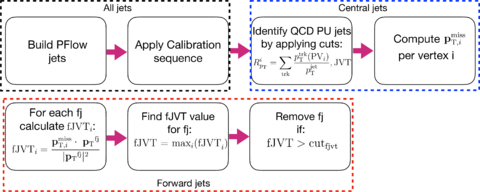
\includegraphics[width=0.8\textwidth]{figures/reco/reco_fjvt.png}
  \caption{The fJVT algorithm using PFlow jets. Taken from Ref.~\cite{ATLAS:2019ecn}.}\label{fig:reco_fjvt}
\end{figure}